% \todo{Rewrite Introduction to match the conclusion and abstract}
\chapter{Introduction}\label{chap:Introduction}
The demand for power to run computational tasks is accelerating. Across vast parts of society the word "algorithm" has been adopted and is an increased part of the everyday life both in front and behind the screens we look at. To support the rising demand, the transistors which do the heavy lifting of storing and computing the singular 0s and 1s, have been stacked closer and closer. Now they are only a few nanometers wide, a size where they are susceptible to quantum effects preventing from becoming much smaller \cite{morton_embracing_2011}. It seems like the computational power of classical computers are about to plateau.

Some large problems like prime factorization or the simulation of quantum many body system can be formulated compactly and run efficiently by considering quantum bits with the ability of being in a super position of 0 and 1 at the same time instead of the classical on/off bit \cite{preskill_quantum_2018}. With basis in this idea, a lot of different implementations of quantum computers are one the way taking many different forms. From singular atoms trapped in an electric field and run by lasers \cite{brown_co-designing_2016} to storing the information in singular photons and applying beamsplitters to alter the state of it\cite{obrien_optical_2007}. In this thesis, we will consider a qubit built of superconducting materials and frozen to just above the absolute zero. \cite{krantz_quantum_2019}

Over the last decade a lot of work has been placed to building suitable circuits to carry quantum information\cite{krantz_quantum_2019}, using microwave pulses to change the information like the transmon \cite{koch_charge_2007} and fluxonium \cite{manucharyan_fluxonium_2009}, and getting multiple qubits to interact with each other \cite{yan_tunable_2018}. With recent progress the ability to do operations on single superconducting qubits \cite{barends_superconducting_2014} has leaped forward. Even multi qubit gates have approached the 99.9 \% fidelity mark\cite{ding_high-fidelity_2023}. While improvements have also been made in initializing and reading out the qubit \cite{walter_rapid_2017, swiadek_enhancing_2023}, this is still a  significant challenge and will be the focus of this thesis.

The state preparation and measurement errors (or SPAM for short) are difficult to separate and is a big hurdle to get over before doing high fidelity quantum algorithms like error-correcting codes on superconducting qubits. By first understanding the physics of a superconducting qubit readout, we will in this thesis built models allowing us to dive deep in how different physical parameters contribute to the SPAM errors.



% In fields with quantum mechanical nature the phase space is exponential and classical computers can only provide limited information in simulations. To overcome this barrier, huge amounts of work, energy and means have been poured into the field of quantum computations. \\
% Quantum computers can take many forms and in its essence the mapping of quantum systems or algorithms onto something of quantum mechanical nature. This can be done on single atoms in ion traps, electron spin caugt in a spin-qubit or superconducting qubits which will be the focus of this project. \\
% In a constant search for improvements, it might be easy to forget, that superconducting quantum computers have already come far and is an excellent place to test the theory of quantum mechanics. In this project, we will step a bit back from the expansion and improvements of the qubits and simply see, how well we can understand a single qubit coupled to a resonator. 

\newpage
\section{Outline of Thesis}
The thesis is built up in the following way. The first few chapter will be theory, in the rest of chapter \ref{chap:Introduction}, we will cover some fundementals of quantum mechanics and in chapter \ref{chap:cQED} we will focus in particular on theory of circuit Quantum Electrodynamics (cQED) and provide a quick overview of the device we use for experiments. Chapter \ref{chap:computations_and_readout} we will go into more depth of how the qubit is coupled to the control hardware to allow control and readout of the qubit. To investigate how interactions with the environment affects our qubit, we will introduce open quantum systems in chapter \ref{chap:open_quantum_systems} and we will in chapter \ref{chap:measurements} we will see how measurements change the dynamics.

With the theory covered, we will in chapter \ref{chap:readout} investigate the performance of readout in our system. In chapter \ref{chap:calibration} we do the necessary experimental calibrations of the system to allow us to built it in simulation, which is done in chapter \ref{chap:model}. Finally, we will in chapter \ref{chap:budget} use our model to investigate how different parameters contribute the readout infidelity by changing them in our model.  



% \todo{Update the outline and write coherently}
% \begin{itemize}
%     \item In the first section, we will review the circuit quantum electrodynamics (cQED) which gives rise to the potentials we base our qubit and readout resonator on.
%     \item We will go into depth of how this system can be viewed in the light of the parameters and limits we impose on the system.
%     \item The thesis will the cover, how our system interacts with the environment. This will give rise to the Lindblad Master Equation and a discussion of decoherence of our quantum system. 
%     \item Then we will go through how the system is measured. For this we will need to go through the (1) the stochastic master equation which arises in continuous measurements, (2) the microwave field which we will see in the drive line and in the resonator, (3) the amplification chain that leads the resonator signal at 10 mK into the lab and (4) how the signal can be read out by either a homodyne or heterodyne measurement.
%     \item A section focusing on how the IQ plane of the resonator can be used to calibrate different errors. We will hopefully be able to separate State Preparation and Measurement errors using the physics happening in the two.
%     \item A part covering the simulations we can put together from the above. How can we use this to best distiguish the $\ket{0}$ and $\ket{1}$ state. 
%     \item Hopefully, this can be followed by a section where we fit the master equation or stochastic master equation to calibrate hamiltonian of the system while measured.
% \end{itemize}

\section{Qubits}
Improvements in the hardware of classical computers come in many different ways: processing speed, size of memory, or faster buzz speed. Ultimately, these improvements increase our capability of storing, messaging or manipulating single entities called bits. Bits are an on/off switch representing a small piece of information normally represented as either being "1" or "0". Combining billions or even trillions of these bits, we can store data, media or even programs.

While most everyday computing tasks can easily be done using these classical computers, some problems scale exponentially and unforgivably when the size of the problem is increased. Among these problems, we find prime factorization, the traveling salesman problem and even just simulating quantum mechanical systems, a challenge which will return multiple times through this thesis.

Instead of building classical computers of exponentially increasing size, quantum mechanics provides a hope to solve these problems by not going up in size but instead changing the ideas of the bit. More specifically, the quantum bit (qubit) is not bound by the discreteness of the classical bit but can be in some combination (or superposition) of "0" and "1" at the same time \cite{krantz_week_2019}.

\subsection{A Quantum Mechanical State}
In quantum mechanics, our system can live in either a continuous spectrum like the position of a particle or a discrete spectrum like the spin of an electron which either points up or down. When considering a quantum mechanical object, all possible physical configurations span a Hilbert Space of infinite or finite dimensions. One of these configurations containing all the information one could measure is an element in the Hilbert space and is called a quantum mechanical state, mathematically represented with a ket $\ket{\psi}$. \cite{sakurai_modern_2021}

The observable information about the state of the system can be found by applying operators to it. Applying an operator is represented by multiplication from the left: $A\ket{\psi}$. Of special interest are eigenstates to the operator, which are states satisfying $A\ket{a} = a \ket{a}$, where $a$ is the eigenvalue and $\ket{a}$ is the eigenstate. The energy of the system is an observable which can be measured with the Hamiltonian operator. In classical mechanics the Hamiltonian generates equations of motion and it play the same role in quantum mechanics. \cite{sakurai_modern_2021}

\subsection{The Two Level System}\label{sec:tls}
In creating a qubit, we need a quantum mechanical two level system where one state can be the "0" and one be the "1". There are two ways of achieving this: first, we could use an object living in a 2-dimensional Hilbert space like the spin of an electron. Here we could encode "1" to the spin up state and "0" to be spin down. 

The other way is to limit ourselves to a subspace of a larger Hilbert space. Since the quantum mechanical states are subject to Boltzmann statistics \footnote{That is the relative probability of finding a qubit in two different states (say $\ket{1}$ and $\ket{0}$) can be found as the fraction between their Boltzmann factor: $e^{-E_1 / k_b  T} / e^{- E_0 / k_b  T}$.}, if we go to low enough temperatures (that is the difference in energy $\Delta E \gg k_b T$)  the system will primarily occupy the lowest energy states. 

When the two states of the system are described as $\ket{0}, \ket{1}$, we can construct a superposition of these two:
\begin{equation}
    \ket{\psi} = a \ket{0} + b \ket{1}
\end{equation}
where a and b are complex numbers. Normalizing and using the freedom to choose a global phase, we can write the general state of a two level system up as:
\begin{equation}\label{eq:general_2_state}
    \ket{\psi} = \cos (\theta / 2) \ket{0} + e^{i\phi}\sin(\theta / 2)\ket{1}
\end{equation}
Where we end up with the two angles $\theta$ and $\phi$ which respectively determining the relative occupation in these two states and a phase between them. With these two angles, it is convenient to represent a qubit geometrically.

\subsection{The Bloch Sphere}
\begin{marginfigure}[3 cm]
    \centering
    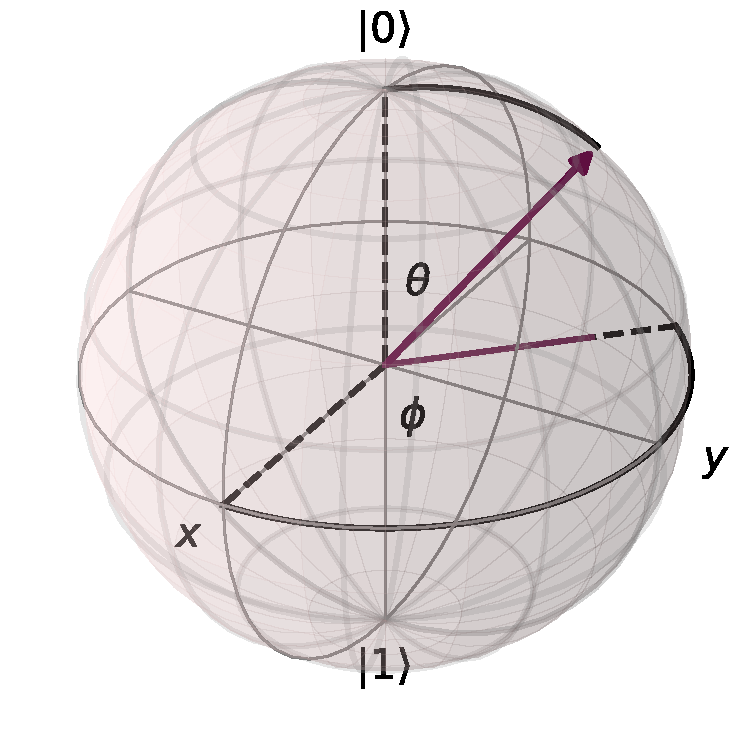
\includegraphics[]{Figs/Theory/bloch_sphere.pdf}
    \caption{Representation of a qubit state on the Bloch sphere. The angles $\phi$ and $\theta$ are displayed along with the projection onto the x-y plane.}
    \label{fig:bloch_sphere}
\end{marginfigure}
With the two angles $\theta$ and $\phi$ and a normalization requiring a length of 1, the two angles can be visualized as a vector pointing to a unit sphere. When representing a general two level state, we call it a Bloch Sphere and a representation can be seen in fig \ref{fig:bloch_sphere}.

On the Bloch Sphere, the state $\ket{0}$ will be positive along the z-axis and $\ket{1}$ in the negative direction. with this mapping the projection of the state vector unto the z-axis gives the probabilities of finding $\ket{0}$ or $\ket{1}$ respectively. The x-y plane is determined by the $\phi$ component and will be the phase difference between the two states. \cite{krantz_week_2019}


% \section{Time Evolution of a Quantum System}
% As a physics student, one is often met early in ones career by Newtons second law, stating that acceleration equals force times mass $\Vec{F} = m \Vec{a}$. Knowing the force asserted on an object thus gives the equations of motion. Often it is however more beneficial to represent the equations of motions in the Hamiltonian formalism, where one can derive the equations of motion by the energy of the system (the Hamiltonian). The equation of motions are now given by a coordinate and the canonical momentum to that coordinate. 

% In this formalism the time dependence of the coordinates $q$ and canonical momentum $p$ is given by\footnote{The canonical momentum is found from the Lagrangian which is related to the Hamiltonian by a Legendre transformation} :

% \begin{align}
%     \dot{p} = - \pfrac{}{q} &H(p, q) \\
%     \dot{q} = \pfrac{}{p} &H(p, q)
% \end{align}

% Or for a general function of a set of coordinates and the set of canonical momenta $f(\{q_i\}, \{p_i\}, t)$, we can represent the time-dependence using Poisson brackets: \cite{Fetter_continous_mechanics}
% \marginnote{A Poisson bracket refers to a specific combination of differentials. With $\{F, G\} = \sum_i \left(\pfrac{F}{q_i} \pfrac{G}{p_i} - \pfrac{F}{p_i} \pfrac{G}{q_i} \right)$} 

% \begin{equation}
%     \dot{f} = -\{H, f\} + \pfrac{}{t} f 
% \end{equation}

% \paragraph{Going Quantum - }
% From the Hamiltonian formalism the switch to quantum mechanics is significantly shorter. By first introducing the commutator between two operators: \todo{Introduce operators above with operators and uncertainty principle}
% \begin{equation}
%     \comm{A}{B} = AB - BA
% \end{equation}

% Now making the mapping from Poisson brackets to commutators with the appropiate prefactor, we find the correspondence principle:

% \begin{equation}
%     \{A, B\} \to \frac{\hbar}{i} \comm{A}{B}
% \end{equation}

% Such that the time dependence of an operator is given by:
% \begin{equation}
%     \dot{A} = \frac{i}{\hbar} \comm{H}{A} + \pfrac{}{t} A
% \end{equation}

% \textbf{Get to Schödingers Equation here}

% \textbf{Maybe introduce like this instead} \\ \noindent
\section{Time Evolution of a Quantum System}
Since all states are normalized, a transformation from into another must leave the inner product unchanged. In linear algebra, this is exactly a property of the unitary transformation \footnote{For unitary transformations we have: $\braket{\psi}{\psi} = \mel{\psi}{\unitary^\dagger \unitary}{\psi}$}. So to go from a state at time $t = t_0$ to a later time $t = t_0 + \Delta t$ we wish to find a unitary operator, $\mathcal{U}(\Delta t)$. To keep normalization, the transformation should satisfy:
\begin{equation}
    \braket{\psi; t_0}{\psi; t_0} = \braket{\psi; t_0 .. \Delta t}{\psi; t_0 .. \Delta t} = \mel{\psi; t_0}{\unitary^\dagger (\Delta t) \unitary(\Delta t)}{\psi; t_0} 
\end{equation}
which is satisfied since $\unitary$ is unitary and $\unitary^\dagger (\Delta t) \unitary(\Delta t) = \identity$. In addition, we would like the state to remain unchanged if no time has passed such that $\unitary(\Delta t) \to \identity$ when $\Delta t \to 0$. For an infinitesimal time step, the two conditions are satisfied by taking the unitary to linear order:
\begin{equation}\label{eq:infinitesimal_time_evolution}
    \unitary(dt) = \identity - i \Omega dt
\end{equation}
Where $\Omega$ is a hermitian operator with units of frequency. \footnote{This formkeeps the normalization since $\unitary^\dagger(dt)\unitary(dt) = (\identity + i \Omega dt)(\identity - i \Omega dt) = \identity + dt^2 \Omega^2$ which goes to identity in the limit of $dt \to 0$ the $dt^2$ term vanishes.}
Since the Hamiltonian in classical mechanics are a generator of time evolution it is not so strange that it turns out to be of quantum mechanics as well. The actual operator is $\Omega = \frac{H}{\hbar}$. For eq. \ref{eq:infinitesimal_time_evolution} and by defining $\ket{\psi; t..dt} - \ket{\psi; t} = d\ket{\psi; t}$ we find the Schrödinger equation by:
\begin{align}
    \ket{\psi; t..dt} &= \unitary(dt) \ket{\psi; t} = \left(\identity - i \frac{H}{\hbar}   dt\right) \ket{\psi} \\
    \ket{\psi; t..dt} - \ket{\psi; t} &= i \frac{H}{\hbar}   dt \ket{\psi} \\
    i \hbar \frac{d}{dt}\ket{\psi} &=  H \ket{\psi}
\end{align}
Which is known as the Schrodinger's equation and governs unitary time evolution of quantum mechanical system given that it is closed from the environment and is not measured \cite{sakurai_modern_2021}. Two problems which we will return to in great detail.

If the Hamiltonian is independent of time, we can express the time evolution operator as:
\begin{equation}
    \unitary(\Delta t) = e^{-iH\Delta t/\hbar}
\end{equation}
which entirely removes the time-dependence from the state such that $\ket{\psi; t} = \unitary(t)\ket{\psi; t = 0}$.
If on the contrary, the Hamiltonian is dependent on time and commutes at different times, we can write it as:
\begin{equation}
    \unitary(\Delta t)\ket{\psi; t_0} = \exp\left(-\frac{i}{\hbar}\int_{t_0}^{t_0 + \Delta t} dt H(t)\right)\ket{\psi; t_0}
\end{equation}
If the Hamiltnoian at different times do not commute with itself, one could introduce the Dyson series\cite{sakurai_modern_2021}. However, in this thesis we will instead solve the differential equation numerically.

\subsection{Numerical Implementations}\label{sec:numerical_implementations}
The Schrodinger equation gives a simple linear relation between the time derivative and the state, so if we naively were to let $dt\to\Delta t$ and represent the states and the Hamiltonian as vectors and a matrix, we could simply update the state by:
\begin{equation}
    \Vec{\psi}(t + \Delta t) =  \Vec{\psi}(t) - \frac{i\Delta t}{\hbar}\boldsymbol{H} \Vec{\psi}(t)
\end{equation}
and repeat iteratively to get the state at each time step. While this method (Euler integration) is simple to implement it loses precision quickly if the time steps become too large. Since our physical state has to be normalized to be physical, we have to be aware of these numerical instabilities and look into more sophisticated integration algorithms.


\begin{marginfigure}
    \centering
    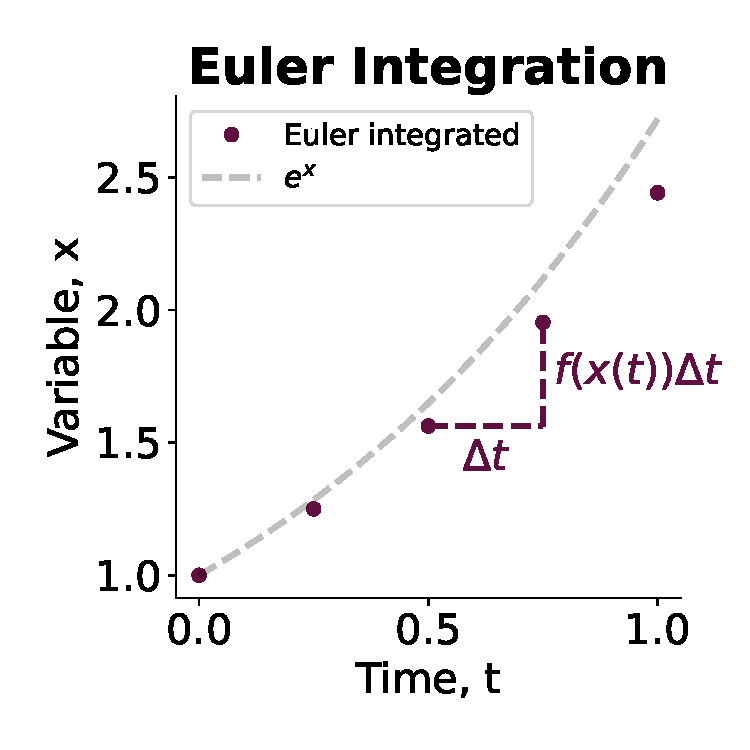
\includegraphics[]{Figs/Theory/euler_integration.pdf}
    \caption{Example of Euler integration $x'(t) = x$}
    \label{fig:Runge-Kutta}
\end{marginfigure}


The method used in the Qutip library \cite{johannson_qutip} is the Adams method. Here we will consider the last $n$ points in order to also approximate the differentials. Consider the differential equation:
\begin{equation}
    y'(t) = f(y(t))
\end{equation}
We could approximate the point $y(t+\Delta t)$ by a taylor series:
\begin{equation}
    y(t) + \Delta t y'(t) + \frac12 \Delta t^2 y''(t) + \frac{1}{3!} \Delta t^3 y'''(t)\dots 
\end{equation}
The idea in the Adams algorithm is to approximate the differential up to order $n$ by using finite difference methods. Then we would have the first two terms simply by:
\begin{equation}
    y'(t) = f(t), \quad y''(t) = \frac{f(t) - f(t - \Delta t)}{\Delta t} 
\end{equation}
And we could combine them to get higher order like
\begin{equation}
    y'''(t) = \frac{y''(t) - y''(t-\Delta t)}{\Delta t} = \frac{y(t) - 2y(t-\Delta t) + y(t-2\Delta t)}{\Delta t^2}
\end{equation}
and beyond. This computation more precise since it takes considers higher order terms up to order $n$ and goes fast since it reuses the old points and just have to do one operation\footnote{in the sense that no operation has to wait for another operation before it can be run.} for the next points. In Qutip $n=12$ by default. One challenge is that the algorithm requires $n$ points to get started. Thus we can either assume that every differential beyond order $m$ is $0$ when calculating the $0$th point. Such that we effectively would do an Euler integration for the first point, a second order Adams for the second and so on. Or, we can use another algorithm which moves forward in time to approximate the higher order differentials. As an example, the Runge-Kutta algorithm can be used.

\todo{Check with source here: https://link.springer.com/book/10.1007/978-3-540-78862-1 should be accessible within KU }



\begin{marginfigure}
    \centering
    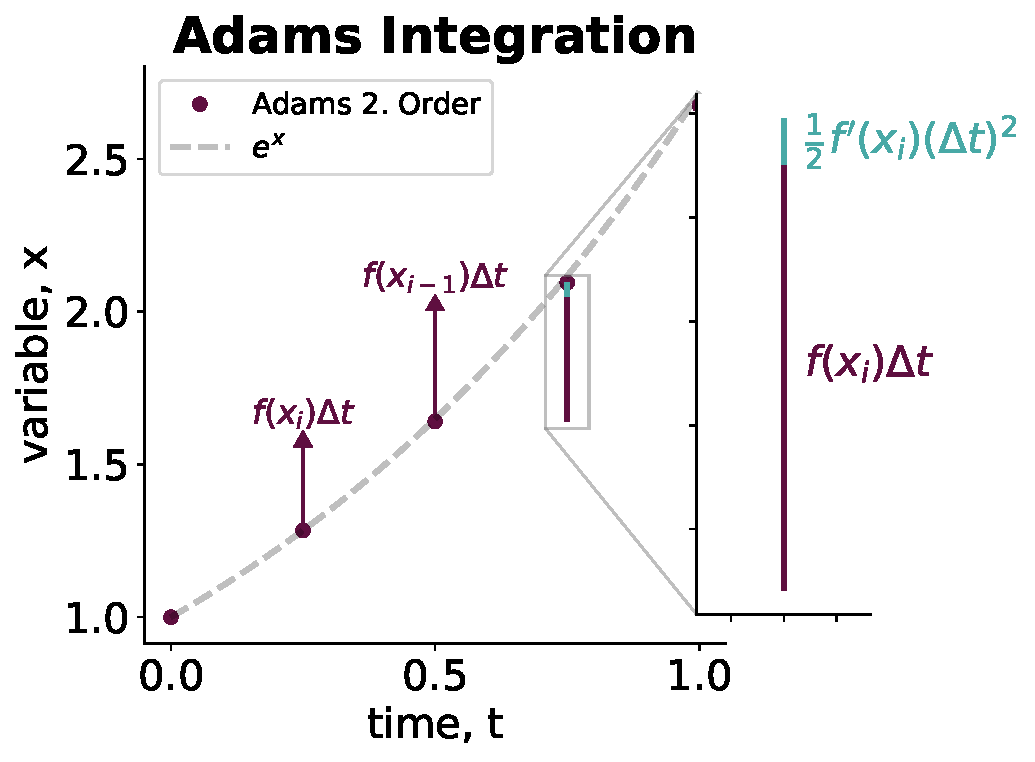
\includegraphics[]{Figs/Theory/adams_intergation.pdf}
    \caption{How the Adams algorithm works. Here the second order derivative is found by the finite difference method to be $f'(x_i) = (f(x_i) - f(x_{i-1}))/\Delta t$}
    \label{fig:Adams integration}
\end{marginfigure}

The Runge-Kutta method is doing this by doing an (or several) intermediate steps to have a trial point. The results can then be combined to make the errors cancel out. To second order, the Runge-Kutta algorithm simply calculates a middle step by doing half a time step: $k_1 = \Delta t / 2 \psi $takes $\Vec{\psi_i} = \Vec{\psi_{i-1}} + k_1 + \mathcal{O}(\Delta t^3)$. To higher orders this lets us suppress the error for the first few steps using multiple steps with the Runge-Kutte method and when we have the first $n$ values, we can switch to the Adams method to improve speed while keeping the error small. \todo{Same source as above? } 
% \todo{Write this properly}
% \paragraph{Adams method} includes the values calculated in the last few steps to determine a polynomial expansion. This does not require to calculate as many points as the Runge-Kutta and comes with a high precision as well. Requires a few points to start, but one could use Runge-Kutta to find the first few points or run the algorithm backwards in time. 


% The Adam package is also the one used in the Qutip package which is used for this thesis. Here the algorithm is run to 12 order with a set error tolerance and the possibility to adapt and take multiple steps between the desired resolution.

\section{Computational Framework of the Thesis}
It is by no means a new idea to solve quantum mechanical problems by numerical simulations, so multiple nice modules exists. In this thesis, we base most of our calculations on the integration method present in the Qutip Library \todo{cite Qutip}. To make faster progress and hopefully contribute to the software in the laboratory, a module to make numerical superconducting qubit experiments was developed during this project. The package is a wrapper around the Qutip Library, but eases the setup of of hamiltonians from typical superconducyying qubits, simulations and data managementS. The documentation for the module QuantumDeviceSimulation can be found in the appendix or at the following website. \todo{Link to the documentation in appendix and on the webs.}

An overview of the module is shown in figure \ref{fig:module_overview}. In general, it is built in three main parts:
\begin{itemize}
    \item \textbf{Devices} which are the physical devices placed in the system. This includes different Qubits, resonators and pulses.
    \item \textbf{Systems} are combinations of devices along with descriptions of how they interact.
    \item \textbf{Experiments} are organizing the different sweeps of parameters and applying the proper integration. 
\end{itemize}

\begin{figure*}
    \centering
    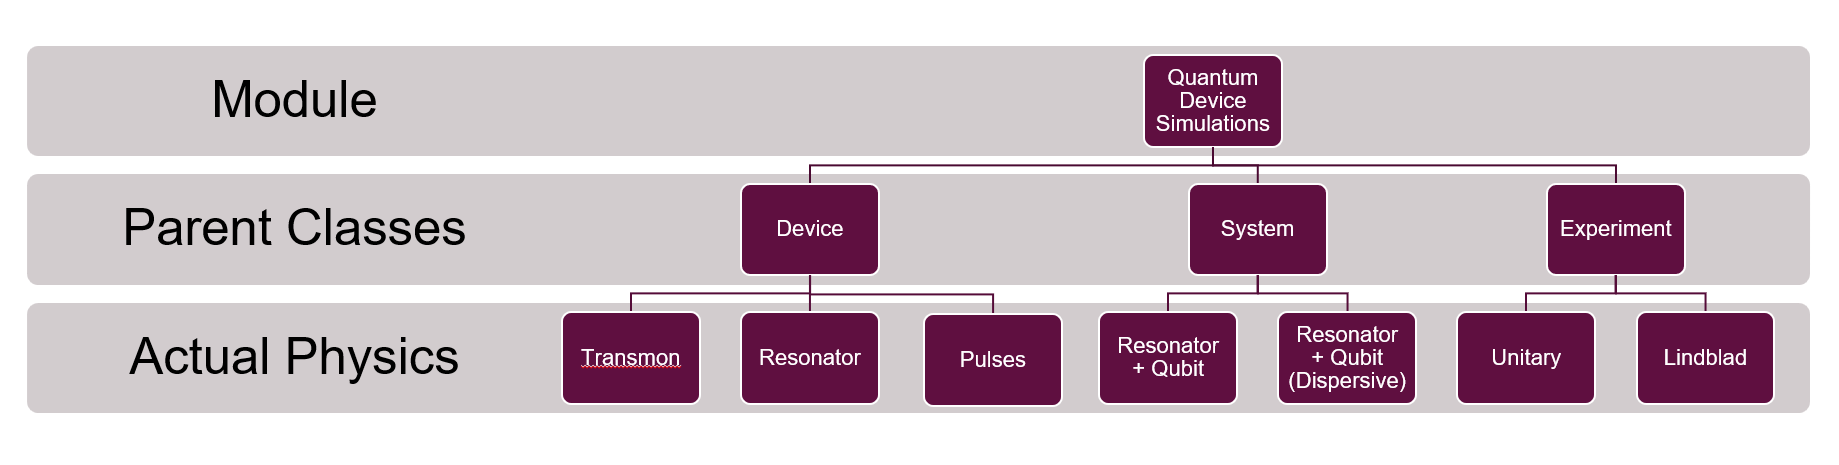
\includegraphics{Figs/Sections/Introduction/module.png}
    \caption{Module structure.}
    \label{fig:module_overview}
\end{figure*}
\todo{Add a final structure and describe properly in caption}